\chapter{Diseño técnico}

En este capítulo analizaremos los requisitos de la aplicación previamente al inicio de su implementación.

\section{Listado de historias de usuario (Backlog)}

Para extraer las historias de usuario se ha usado la aplicación \textbf{Jira}\footnote{\url{https://www.atlassian.com/software/jira}}, de la compañía \textbf{Atlassian}. Por consistencia y aunque puedan parecer desordenados, los identificadores de las épicas y de las historias que aparecen en esta sección son los que se han obtenido en dicha herramienta.

\begin{enumerate}
    \item[MTB-1.] Gestión de agrupaciones.
        \begin{enumerate}
            \item[MTB-8.] Como administrador de una agrupación, quiero crear una nueva agrupación.
            \item[MTB-9.] Como administrador de una agrupación, quiero eliminar mi agrupación.
            \item[MTB-10.] Como administrador de una agrupación, quiero editar mi agrupación.
        \end{enumerate}
    \item[MTB-2.] Gestión de membresías.
        \begin{enumerate}
            \item[MTB-11.] Como administrador de una agrupación, quiero añadir miembros a mi agrupación.
            \item[MTB-13.] Como usuario, quiero unirme a una agrupación.
            \item[MTB-12.] Como administrador de una agrupación, quiero eliminar miembros de la agrupación.
            \item[MTB-14.] Como miembro, quiero salirme de una agrupación.
            \item[MTB-15.] Como miembro, quiero seleccionar qué instrumento toco en la agrupación.
        \end{enumerate}
    \item[MTB-4.] Gestión de eventos.
        \begin{enumerate}
            \item[MTB-16.] Como administrador de una agrupación, quiero añadir un evento.
            \item[MTB-35.] Como administrador de una agrupación, quiero configurar qué miembros están invitados a un evento.
            \item[MTB-17.] Como administrador de una agrupación, quiero editar los datos de un evento.
            \item[MTB-18.] Como administrador de una agrupación, quiero eliminar un evento.
            \item[MTB-19.] Como miembro, quiero ver la lista de eventos a los que estoy invitado.
            \item[MTB-20.] Como miembro, quiero ver los detalles de un evento.
            \item[MTB-36.] Como administrador, quiero publicar un evento.
            \item[MTB-37.] Como miembro, quiero posponer un evento.
        \end{enumerate}
    \item[MTB-5.] Notificaciones.
        \begin{enumerate}
            \item[MTB-58.] Como administrador, quiero ser notificado cuando un miembro registra su asistencia prevista a un evento.
            \item[MTB-26.] Como miembro, quiero ser notificado cuando soy invitado a un evento.
            \item[MTB-27.] Como miembro, quiero ser notificado cuando se modifica un evento.
            \item[MTB-28.] Como miembro, quiero ser notificado cuando se pospone un evento.
            \item[MTB-55.] Como miembro, quiero ser notificado cuando se añada nuevo repertorio.
            \item[MTB-47.] Como miembro, quiero seleccionar qué notificaciones recibo.
        \end{enumerate}
    \item[MTB-21.] Gestión de asistencia.
        \begin{enumerate}
            \item[MTB-22.] Como miembro, quiero registrar mi asistencia prevista a un evento.
            \item[MTB-23.] Como miembro, quiero justificar mi ausencia a un evento.
            \item[MTB-24.] Como administrador, quiero ver qué miembros asistirán a un evento.
            \item[MTB-25.] Como administrador, quiero registrar la asistencia real a un evento.
            \item[MTB-48.] Como administrador, quiero ver un resumen de la asistencia a un evento.
        \end{enumerate}
    \item[MTB-6.] Recordatorios.
        \begin{enumerate}
            \item[MTB-32.] Como miembro, quiero recibir recordatorios de los eventos próximos.
        \end{enumerate}
    \item[MTB-29.] Gestión de administradores.
        \begin{enumerate}
            \item[MTB-30.] Como administrador, quiero hacer que un miembro sea administrador.
            \item[MTB-31.] Como administrador, quiero quitarle a un miembro los permisos de administrador.
            \item[MTB-33.] Como administrador, quiero especificar mi rol como administrador.
        \end{enumerate}
    \item[MTB-3.] Gestión de repertorio.
        \begin{enumerate}
            \item[MTB-34.] Como administrador, quiero añadir repertorio a mi agrupación.
            \item[MTB-45.] Como administrador, quiero editar una obra.
            \item[MTB-46.] Como administrador, quiero eliminar una obra.
            \item[MTB-43.] Como administrador, quiero añadir la partitura de una obra.
            \item[MTB-44.] Como administrador, quiero eliminar la partitura de una obra.
            \item[MTB-49.] Como administrador, quiero añadir un \textit{tag} a una obra.
            \item[MTB-50.] Como administrador, quiero eliminar un \textit{tag} de una obra.
            \item[MTB-56.] Como miembro, quiero descargar las partituras.
        \end{enumerate}
    \item[MTB-59.] Registro de errores.
        \begin{enumerate}
            \item[MTB-60.] Como administrador de sistemas, quiero tener una vista centralizada de los errores que se hayan registrado en la aplicación.
        \end{enumerate}
\end{enumerate}


\section{Historias de usuario}

\section{Metodologías y tecnologías de base que podrían usarse}\label{section:metodologias}

En esta sección haremos una reflexión y análisis sobre las herramientas que usaremos durante el desarrollo, de forma que pueda existir una formación en el uso de estas tecnologías previa al inicio del desarrollo del proyecto.

\subsection{Lenguaje de programación}
Se plantean los siguientes lenguajes de alto nivel, que disponen de \textit{frameworks} implementados para crear un bot de Telegram:

\begin{itemize}
    \item \textbf{JavaScript}: es un lenguaje compilado en tiempo de ejecución, con tipado dinámico y multi-paradigma, soportando programación orientada a objetos, funcional, imperativa y dirigida por eventos\cite{wiki:JavaScript}. Se conforma al estándar ``ECMAScript'', y es una de las tecnologías centrales de la World Wide Web: el 98\% de los sitios web lo usan en el lado del cliente\cite{javascriptUsage}, y desde el surgimiento de Node.js es una tecnología en auge para servidores.
    \item \textbf{TypeScript} (\url{https://www.typescriptlang.org/}): es un superconjunto de JavaScript que añade sintaxis para tipos estáticos, y a través de un compilador genera código JavaScript\cite{typescriptWeb}. El añadido de tipos estáticos permite detectar errores de forma más temprana y agilizar la escritura de código gracias al autocompletado. Por otro lado, la adición de tipos es un tiempo extra empleado por el programador, por lo que debe analizarse si es conveniente su uso o no.
    \item \textbf{Python} (\url{https://www.python.org/}): es un lenguaje interpretado, interactivo y principalmente orientado a objetos, aunque soporta otros paradigmas como el funcional o el procedimental\cite{pythonFAQGeneral}. Es muy usado en el campo de la computación científica y la inteligencia artificial. Su uso en el desarrollo web se ha extendido para el lado del servidor con la aparición de frameworks como Django (\url{https://www.djangoproject.com/}) o Flask (\url{https://flask.palletsprojects.com/}).
    \item \textbf{PHP} (\url{https://www.php.net/}): es un lenguaje interpretado usado principalmente para desarrollo web en el lado del servidor, cuya principal característica es que puede ser embebido en HTML, de forma que cada ``trozo de PHP'' se ejecuta para intercambiarse por HTML. Sin embargo su uso ha cambiado en los últimos años, dando lugar a frameworks como Symphony (\url{https://symfony.com/}) o Laravel (\url{https://laravel.com/}) basados en la arquitectura Modelo-vista-controlador.
\end{itemize}

Se proporciona una tabla comparativa entre los lenguajes, la tabla \ref{tab:comparacionLenguajes}.

\begin{table}
\begin{minipage}{\textwidth}
\begin{tabularx}{\textwidth}{|l|X|X|X|X|}
\hline
   & JavaScript                       & TypeScript             & Python                    & PHP                       \\
\hline
Tipo                                                & Compilado en tiempo de ejecución & Compilado a JavaScript & Interpretado              & Interpretado              \\
\hline
Tipado estático                                     & No                               & Sí                     & Poco estricto, y poco uso & Poco estricto, y poco uso \\
\hline
Coste\footnote{Aprendizaje necesario por parte del autor para poder implementar el proyecto}                                & Nulo                             & Bajo                   & Medio                     & Medio                     \\
\hline
Popularidad\footnote{\url{https://survey.stackoverflow.co/2022/}} & 65.36\%                          & 34.83\%                & 48.07\%                   & 20.87\%                   \\
\hline
Comunidad \footnote{Preguntas totales en stackoverflow: \url{https://stackoverflow.com/tags}}      & 2432281                          & 196707                 & 2035248                   & 1447104               \\
\hline
\end{tabularx}
\end{minipage}
\caption{Comparación de lenguajes de programación}\label{tab:comparacionLenguajes}
\end{table}

\subsubsection{Decisión}

Por el menor tiempo necesario para la formación del desarrollador en los lenguajes \textbf{JavaScript} y \textbf{TypeScript}, se elegirá uno de estos.

\textbf{TypeScript} es de gran ayuda cuando se desarrolla una aplicación compleja y con un solo desarrollador: puede acelerar el desarrollo gracias al autocompletado y evita la mayor parte de los errores en tiempo de ejecución, reduciendo el tiempo necesario para pruebas. Es el lenguaje que usaremos en el proyecto.

\subsection{Framework para el desarrollo del bot}\label{subsection:elegirFramework}

Existen diversas bibliotecas que ayudan a crear un bot, de forma que no haya que escribir todo el código desde cero para interaccionar con la API de Telegram, siguiendo el principio ``Don't Reinvent the Wheel'' (``No reinventes la rueda'') para también ahorrar presupuesto.

Las opciones que se analizan son:

\begin{itemize}
    \item \textbf{Telegraf} (\url{https://telegraf.js.org/}): biblioteca desarrollada inicialmente para JavaScript, migrada en la versión 4 dando soporte a TypeScript. No dispone de documentación guiada, y la migración a la versión 4 trajo consigo más complejidad de uso. Está inspirada el sistema de middleware de Express.\footnote{\url{https://expressjs.com/es/guide/using-middleware.html}}
    \item \textbf{grammY} (\url{https://grammy.dev/}): biblioteca desarrollada desde un inicio para TypeScript (aunque se puede usar con JavaScript). Está inspirada en telegraf y fue creada desde cero por uno de los antiguos mantenedores de Telegraf como única forma de resolver sus mayores inconvenientes\footnote{\url{https://github.com/telegraf/telegraf/discussions/1526}}. Dispone de una completa documentación con guías para cada uno de los conceptos importantes.
    \item \textbf{node-telegram-bot-api} (\url{https://github.com/yagop/node-telegram-bot-api}): biblioteca ligera para interactuar con la API de Telegram, diseñada para Node.js, y no implementa un sistema de middleware.
    \item \textbf{python-telegram-bot} (\url{https://python-telegram-bot.org/}): biblioteca para Python que provee clases de alto nivel como capa de abstracción sobre la API de Telegram.
\end{itemize}

La tabla \ref{tab:comparacionFrameworks} compara los distintos frameworks.

\begin{table}
\begin{minipage}{\textwidth}
\begin{tabularx}{\textwidth}{|l|X|X|X|X|}
\hline
& telegraf & grammY & node-telegram-bot-api & python-telegram-bot \\
\hline
Lenguaje & JavaScript & Typescript & JavaScript & Python \\
\hline
Documentación & Autogenerada, solo API & Completa, numerosos tutoriales & Básica & Autogenerada, solo API \\
\hline
\makecell[l]{Versión API \\Telegram} & 6.2 & 6.2 & 6.2 & 6.2 \\
\hline
Popularidad\footnote{Estrellas en GitHub a 7 de octubre de 2022} & 6.1k & 663 & 6.5k & 19.8k \\
\hline
\end{tabularx}
\end{minipage}
\caption{Comparación de frameworks para creación de bots de Telegram}\label{tab:comparacionFrameworks}
\end{table}

\subsubsection{Decisión}
En base a la decisión anterior sobre el lenguaje de programación, eligiremos \texttt{telegraf}, \texttt{grammY} o \texttt{node-telegram-bot-api}.

Lo primero que consideraremos es el nivel de abstracción de estas librerías. \texttt{Telegraf} y \texttt{grammY} aportan un mayor nivel de abstracción gracias a implementar una arquitectura basada en \texttt{middleware}, muy conveniente para bots complejos.

Una vez sopesado esto, el punto que más pesa es la documentación: mientras \texttt{grammY} aporta una documentación completa y con guías para cada uno de los problemas que se pueden encontrar desarrollando un bot de Telegram, \texttt{telegraf} \textbf{no tiene} ninguna documentación más allá de la autogenerada por los comentarios en su código. Dado que no tenemos ninguna experiencia con ninguna de las herramientas, utilizaremos \texttt{grammY} para asegurarnos que la formación pueda llevarse a cabo sin problemas.

\subsection{ORM: \textit{Object-relational mapper}}

Un \textbf{ORM} es una herramienta que nos permite transformar los registros de la base de datos en objetos del lenguaje de programación que estamos usando y viceversa.

Las más famosas para \textbf{TypeScript} son \textbf{TypeORM}, \textbf{Sequelize} y \textbf{Prisma}. Sin embargo, en este aspecto la decisión es sencilla dado que \textbf{Prisma} es el único los tres con la característica de ser totalmente \textit{type-safe}: ofrece tipado estático para todas las entradas y salidas consultas de la base de datos. Por este motivo \texttt{prisma} se ha erguido como un estándar para el lenguaje \textbf{TypeScript}.

\subsection{Base de datos}

La base de datos es ``una colección compartida de datos lógicamente relacionados, junto con una descripción de estos datos, que están diseñados para satisfacer las necesidades de información de una organización''\cite{alma991009264529704990}.

Por otra parte, el sistema gestor de base de datos (SGBD) es ``un sistema software que permite a los usuarios definir, mantener, crear y controlar el acceso a la base de datos\cite{alma991009264529704990}.

Necesitaremos estas herramientas ya que buscamos un sistema que guarde datos de manera persistente y poder recuperarlos y actualizarlos en cualquier momento.

Se analizan alternativas para bases de datos relacionales, basadas en el concepto matemático de relación, representado por tablas\cite{alma991009264529704990}; y también para bases de datos no relacionales documentales.

\begin{itemize}
    \item Para bases de datos \textbf{relacionales}:
    \begin{itemize}
        \item \textbf{PostgreSQL} (\url{https://www.postgresql.org/}): es un SGBD de código abierto y centrado en la escabilidad.
        \item \textbf{MySQL} (\url{https://www.mysql.com/}): es un SGDB de código abierto desarrollado por Oracle.
        \item \textbf{MariaDB} (\url{https://mariadb.org/}): es un SGDB de código abierto creado por desarrolladores de MySQL como respuesta a la adquisición por parte de Oracle, y con características muy parecidas.
    \end{itemize}
    \item Para bases de datos \textbf{no relacionales}:
    \begin{itemize}
        \item \textbf{MongoDB} (\url{https://www.mongodb.com/}): SGDB de código disponible (no necesariamente de código abierto, por usar una licencia SSPL\cite{ssplLicense}.
        \item \textbf{Firestore} (\url{https://firebase.google.com/docs/firestore}): incluido en la suite de servicios ``Firebase'' de Google destinada a la gestión rápida y centralizada de aplicaciones.
    \end{itemize}
\end{itemize}

\subsubsection{Decisión}

El modelo de base de datos que se propone es puramente relacional, por lo que usaremos una base de datos relacional.

Puesto que las diferencias son pequeñas entre las distintas opciones de base de datos relacional y la documentación de \textbf{Prisma} está mayormente basada en PostgreSQL, se escoge esta opción.

\subsection{Servidor virtual}\label{subsection:elegirCloud}
Entre los proveedores que ofrecen servicios gratuitos de computación en la nube se encuentran:

\begin{itemize}
    \item \textbf{DigitalOcean} (\url{https://www.digitalocean.com/}) ofrece 200\$ gratuitos a estudiantes para desplegar servidores privados y servicios de almacenamiento. Además, dispone de servidores preconfigurados, como el que incluye \texttt{docker} preinstalado\footnote{\url{https://marketplace.digitalocean.com/apps/docker}}.
    \item \textbf{Heroku} (\url{https://www.heroku.com/}) tiene la desventaja de que no permite desplegar directamente infraestructura configurada con \texttt{docker compose}. Ofrece 14\$ al mes gratuitos para estudiantes.
    \item \textbf{Microsoft Azure} (\url{https://azure.microsoft.com/}), \textbf{Amazon Web Services} (\url{https://aws.amazon.com/}) o \textbf{Google Cloud} (\url{https://cloud.google.com/}) son plataformas usadas por grandes empresas, con configuraciones muy completas y con gran variedad de servicios. Solo \textbf{Azure} ofrece un plan gratuito para estudiantes.
\end{itemize}

\subsubsection{Decisión}

Hemos probado a configurar el plan gratuito de \textbf{Microsoft Azure} para crear un servidor, pero hemos encontrado numerosos errores y un panel de configuración caótico y lleno de opciones que no necesitamos, por lo que optaremos por \textbf{DigitalOcean}.


\subsection{Almacenamiento de archivos}

Para guardar las partituras de los usuarios necesitaremos un servicio donde almacenarlas. Los servicios más extendidos para guardar archivos de usuarios se denominan de \textbf{almacenamiento de objetos}: ``es una tecnología que almacena y administra datos en un formato no estructurado denominado objetos. [...] Los sistemas de almacenamiento de objetos en la nube distribuyen estos datos a través de varios dispositivos físicos, pero permiten a los usuarios acceder al contenido de forma eficiente desde un único repositorio de almacenamiento virtual''\cite{whatIsObjectStorage}.

Existen varias alternativas de distintos proveedores como \textbf{Amazon S3}\footnote{\url{https://aws.amazon.com/s3}}, \textbf{DigitalOcean Spaces}\footnote{\url{https://www.digitalocean.com/products/spaces}} o \textbf{Google Cloud Storage}\footnote{\url{https://cloud.google.com/storage}}.

\subsubsection{Decisión}

Escogeremos la alternativa de \textbf{DigitalOcean} ya que utiliza la misma API que \textbf{Amazon S3} y nos permitirá tener la administración del servidor y del almacenamiento de archivos centralizada en un mismo panel de control además de utilizar los créditos gratuitos.

%\subsection{Gestor de paquetes}
%\begin{itemize}
%    \item npm
%    \item yarn
%    \item pnpm
%\end{itemize}

\subsection{Documentación}\label{subsection:decisionDocumentacion}

Existen numerosas herramientas para generar páginas web de documentación.

\begin{itemize}
    \item \textbf{GitBook} (\url{https://www.gitbook.com/}): añade estilos a los \texttt{README.md} de \textbf{GitHub}. No permite por tanto crear una \textit{Landing Page} personalizada sino que solo genera páginas de documentación. Un ejemplo creado con \textbf{GitBook} es \url{https://zod.dev/}.
    \item \textbf{Docusaurus} (\url{https://docusaurus.io/}): se basa en la biblioteca para interfaces de usuario \texttt{react}, y permite crear múltiples páginas además de la documentación. Un ejemplo es \url{https://trpc.io/}.
    \item \textbf{VuePress} (\url{https://vuepress.vuejs.org/}): Muy parecido a \textbf{Docusaurus}, pero basado en la biblioteca \texttt{vue} en lugar de \texttt{react}. La documentación de \textbf{grammY} (\url{https://grammy.dev/}) está creada con esta biblioteca.
\end{itemize}

\subsubsection{Decisión}

Solo podremos desarrollar una \textit{landing page} personalizada con \textbf{Docusaurus} o \textbf{VuePress}. Dado que el desarrollador tiene experiencia con \texttt{react}, escogeremos \textbf{Docusaurus} para disminuir el tiempo necesario de formación.

\section{Modelo de la base de datos}

Teniendo claros los requisitos del sistema, podemos analizar la información que necesitaremos representar en la base de datos.

Se propone el modelo relacional de la figura \ref{fig:modeloBaseDatos}, con un total de 11 tablas. La tabla \texttt{Session} se queda aislada ya que será utilizada para guardar las sesiones de los usuarios, y la tabla debe tener un esquema específico para poder usarla automáticamente con el adaptador como se explicará en la sección \ref{subsection:adaptadorPrisma}.

Este modelo es el necesario para implementar todas las historias de usuario que se han extraído, incluidas las que se plantean como tareas futuras a la entrega de este trabajo.

El diagrama se ha realizado con la herramienta \url{https://dbdiagram.io/}.

\begin{figure}[h]
\centering
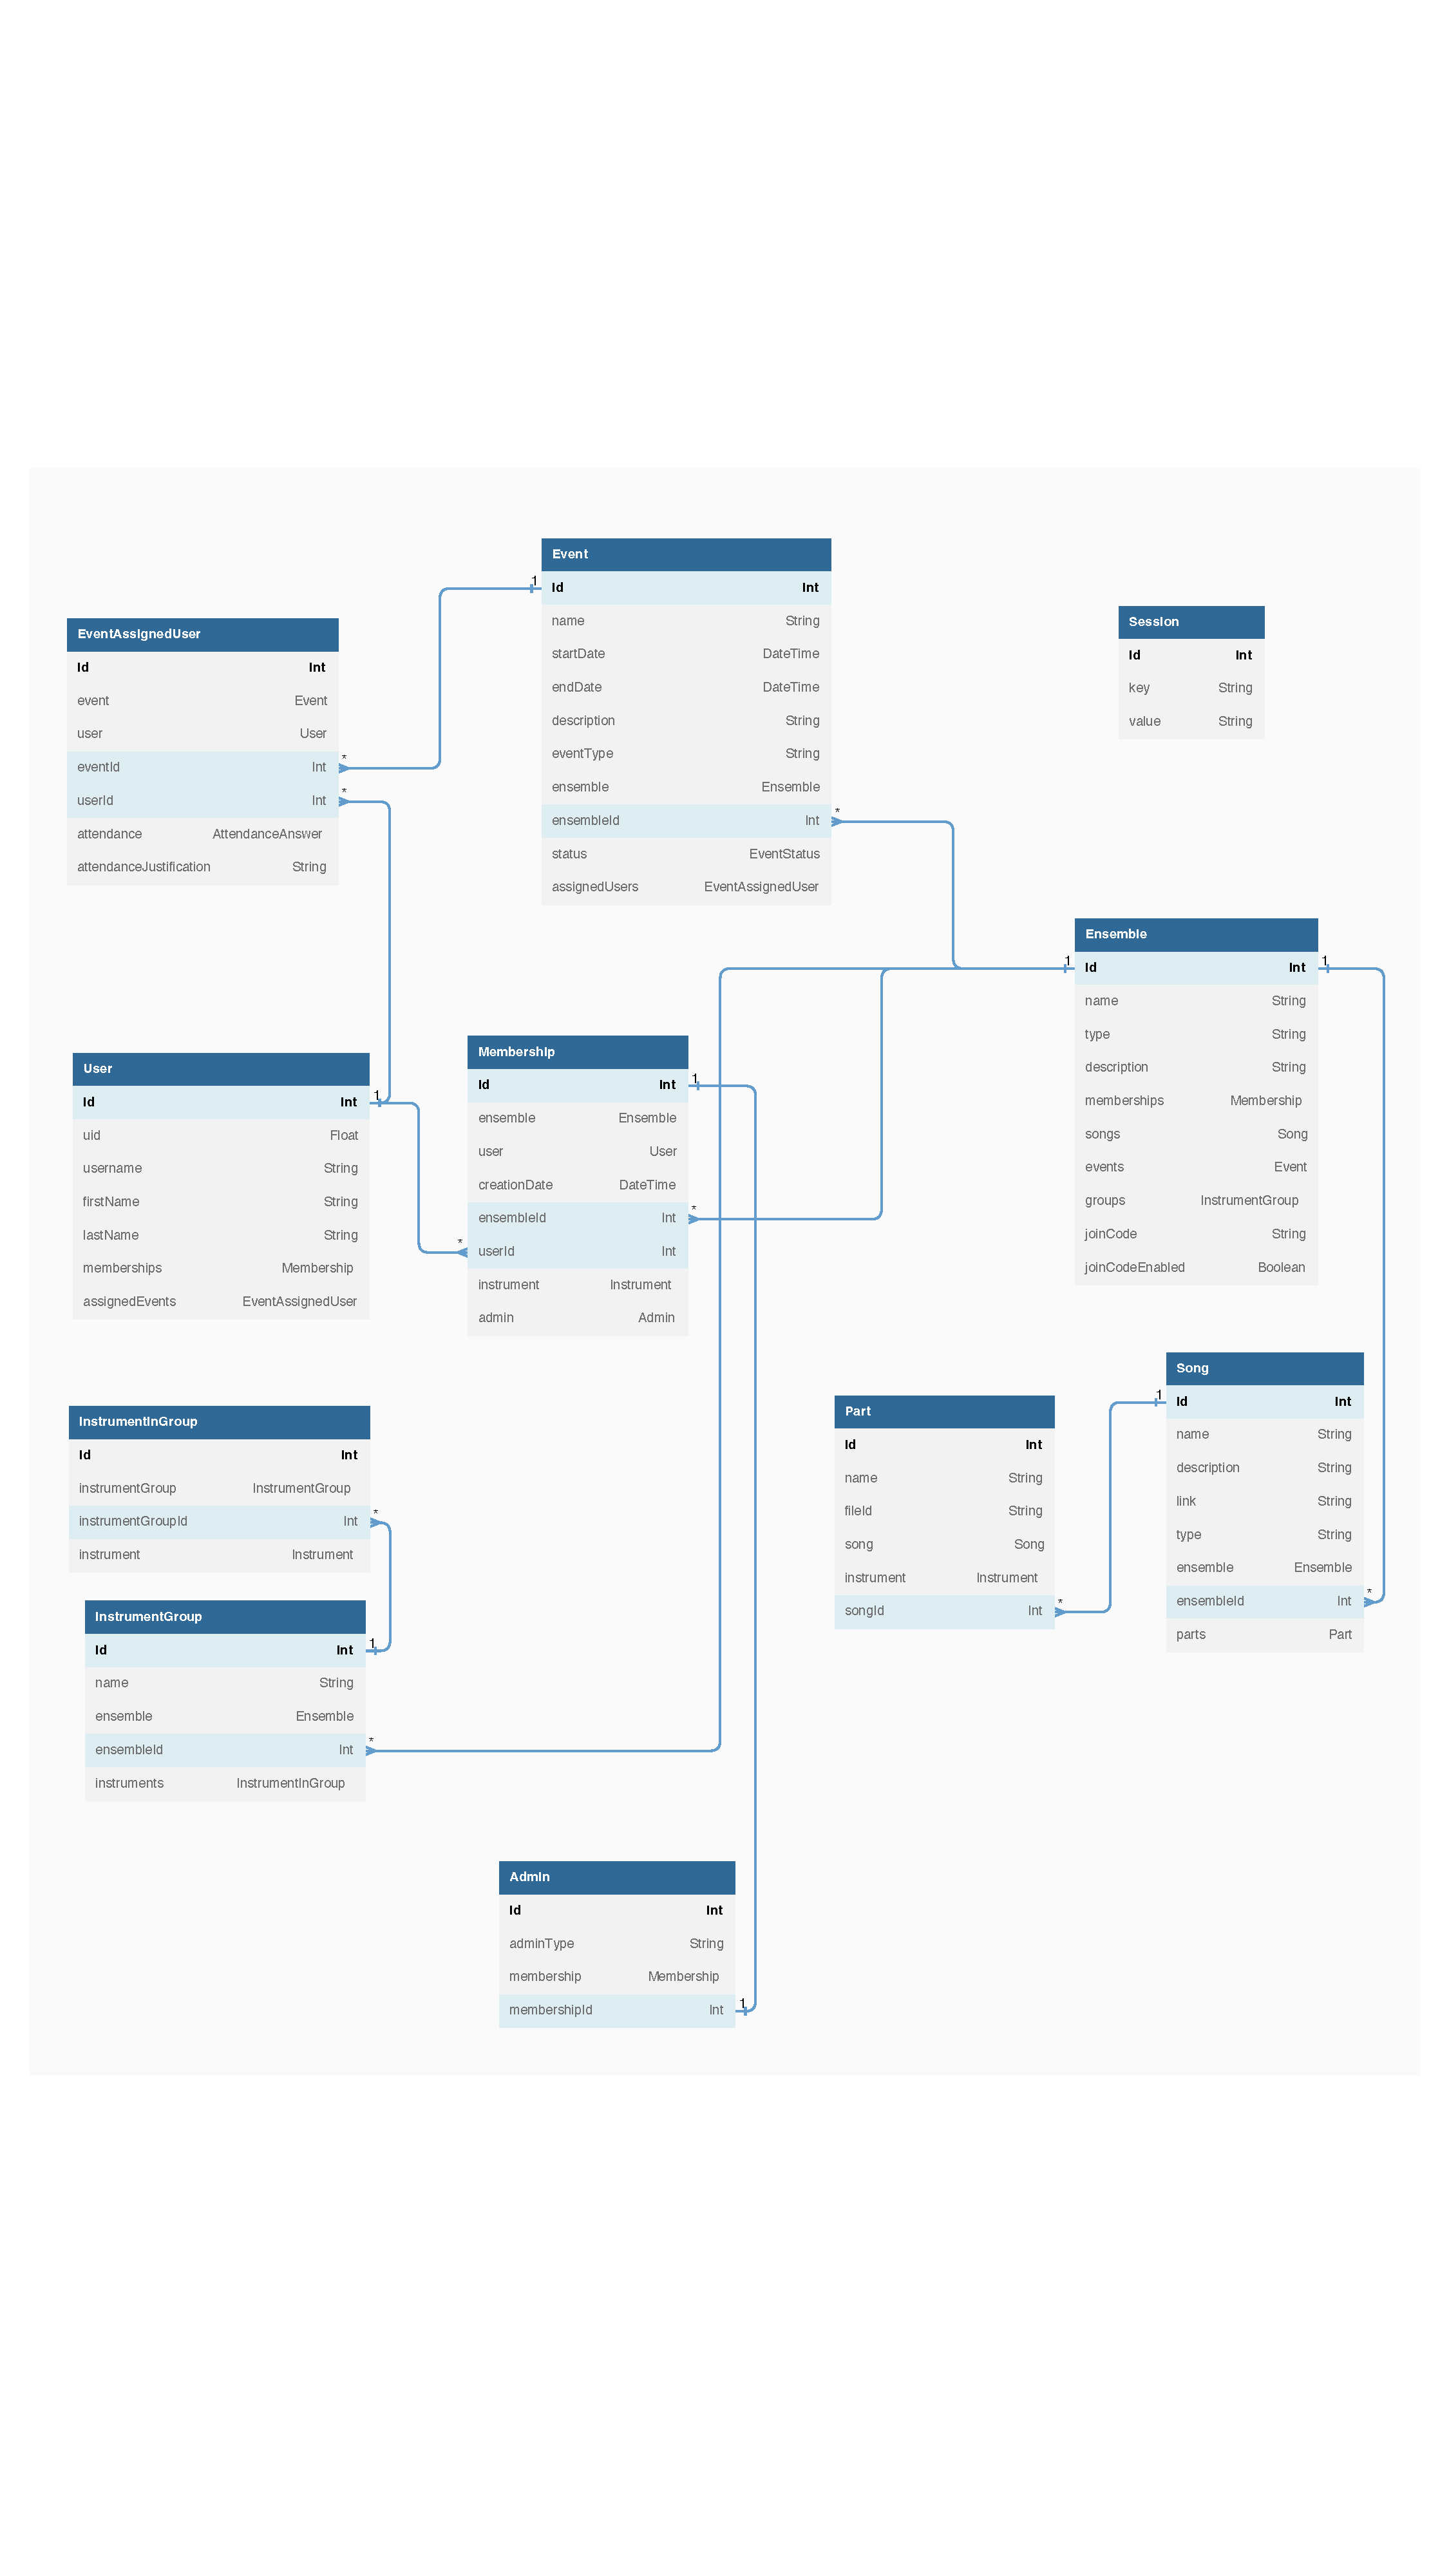
\includegraphics[width=\textwidth]{imagenes/disenyo_tecnico/mordente-db.pdf}
\caption{Modelo de la base de datos}
\label{fig:modeloBaseDatos}
\end{figure}

\section{Arquitectura de Mordente}

Expliquemos la arquitectura del sistema en dos pasos:

\subsection{Arquitectura entre puntos}

Con la arquitectura entre puntos nos referimos a la visualización a alto nivel de las distintas partes físicas necesarias para que nuestra herramienta funcione.

En nuestro caso, existen tres partes claramente diferenciadas:

\begin{itemize}
    \item \textbf{El dispositivo del usuario}, o también llamado cliente. Tiene instalada la aplicación de Telegram, y se comunica bidireccionalmente con los servidores de Telegram para enviar y recibir mensajes.
    \item \textbf{Los servidores de Telegram}. Actúan como intermediarios entre distintos usuarios, así como entre los usuarios y nuestro bot.
    \item \textbf{El bot}. Es un programa que se comunica con los servidores de Telegram para enviar y recibir mensajes, tal y como los clientes, aunque con ciertas diferencias de funcionamiento con los clientes. Este programa puede estar alojado en cualquier ordenador, y en nuestro caso estará alojado en un servidor privado virtual.
\end{itemize}

Esta arquitectura está representada en la figura \ref{fig:arquitecturaPuntos}.

\begin{figure}[h]
\centering
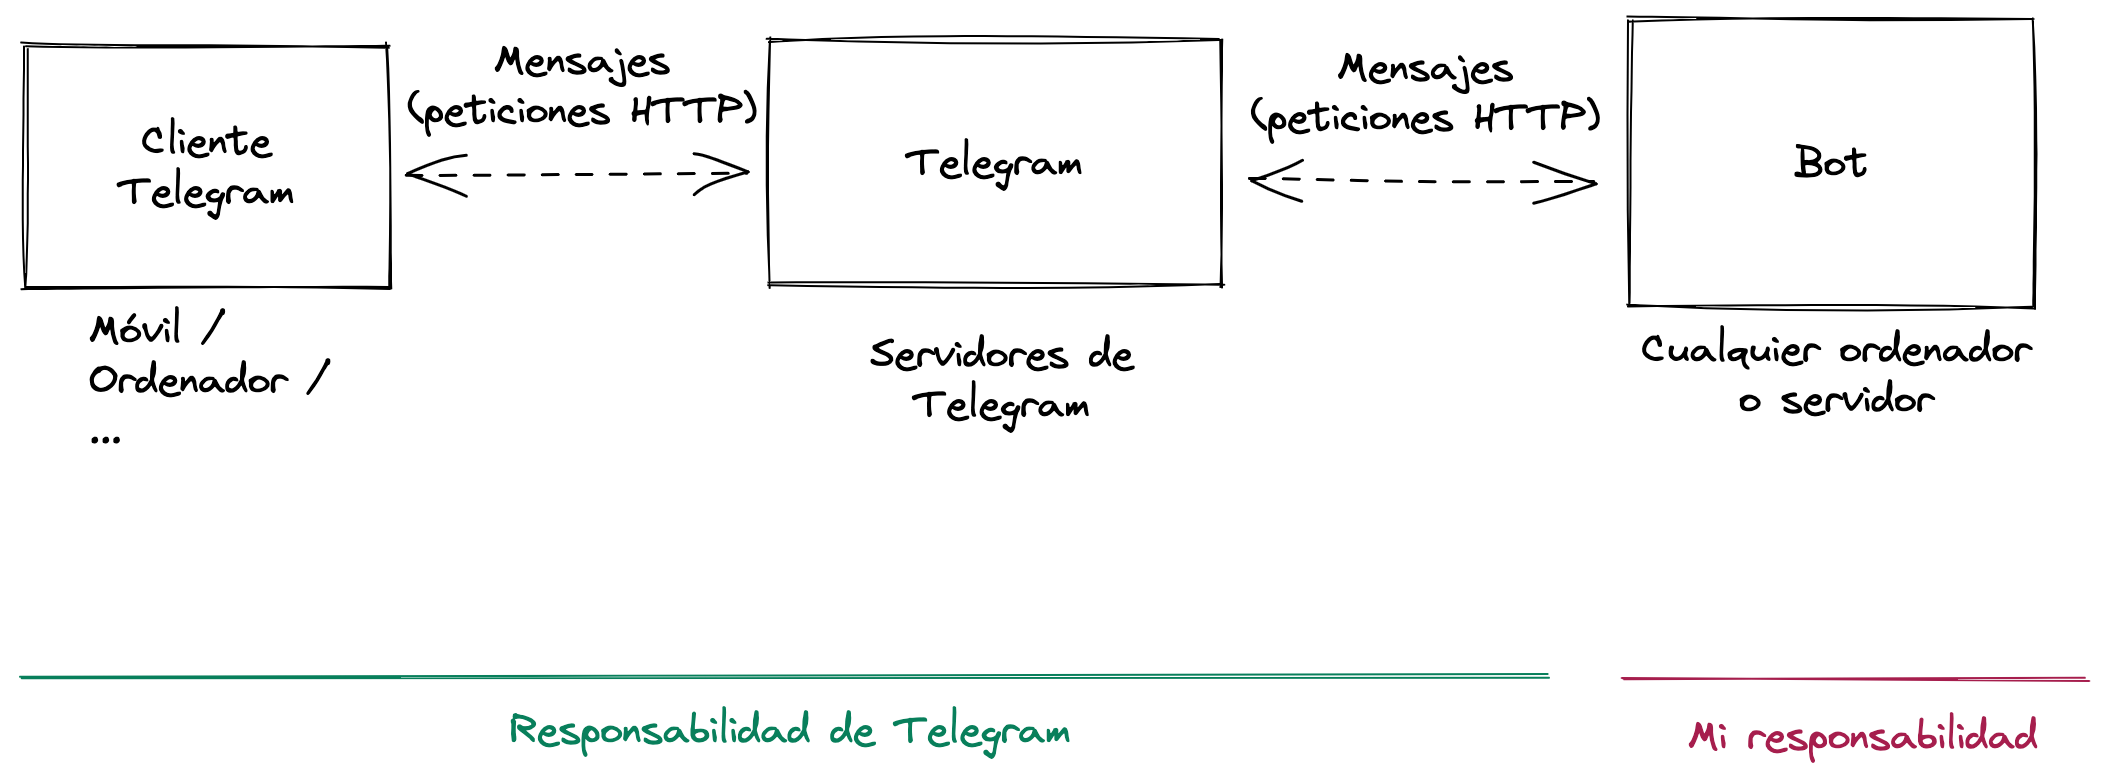
\includegraphics[width=1\textwidth]{imagenes/disenyo_tecnico/arquitectura_puntos.png}
\caption{Arquitectura entre puntos}
\label{fig:arquitecturaPuntos}
\end{figure}

Es importante entender que la única responsabilidad que nos corresponde a nosotros es la de desarrollar la última parte: el bot. El cliente y los servidores de Telegram son partes externas fuera de nuestra responsabilidad, lo cual es una de las ventajas de desarrollar un servicio de este tipo.


% VPS   <->   Telegram API   <->    Telegram Client


\subsection{Arquitectura entre servicios}\label{subsection:arquitecturaServicios}

Para la funcionalidad que necesitamos, el bot debe estar compuesto por varios microservicios a su vez: 

\begin{itemize}
    \item \textbf{El propio bot:} es el microservicio donde implementaremos la comunicación con los servidores de Telegram para recibir mensajes, procesarlos y responderlos adecuadamente.
    \item El bot realiza peticiones a una \textbf{base de datos} donde almacenaremos de forma persistente los datos de los usuarios. Esto garantizará que no perdamos información cuando el bot se reinicie.
    \item Opcionalmente, podremos añadir un microservicio encargado de realizar una \textbf{copia de seguridad} periódica de la base de datos.
    \item Por otro lado tendremos un servicio de \textbf{almacenamiento de archivos} para guardar las copias de seguridad y otros archivos (en nuestro caso, las partituras).
\end{itemize}

En la figura \ref{fig:arquitecturaServicios} se puede visualizar la arquitectura entre los distintos servicios.

\begin{figure}[h]
\centering

\includegraphics[width=\textwidth]{imagenes/disenyo_tecnico/arquitectura_servicios.png}
\caption{Arquitectura entre servicios}
\label{fig:arquitecturaServicios}
\end{figure}

\subsubsection{Localización de los servicios}

Con respecto a dónde disponer los distintos servicios, existen al menos dos opciones: una es alojarlos en el propio servidor que gestionaremos nosotros y cuyos microservicios podremos levantar en un solo paso usando \textit{Docker Compose}\footnote{\url{https://docs.docker.com/compose/}}, y otra es utilizar servicios auto-gestionados por plataformas externas. Hagamos una reflexión para cada uno de los servicios:

\begin{itemize}
    \item El \textbf{bot} puede estar en un servidor propio o en un servicio gestionado, ambas opciones son válidas. La ventaja de tenerlo en el servidor propio será la mayor cercanía posible con la base de datos, resultando en una mayor velocidad de respuesta. La ventaja de utilizar un servicio gestionado es la mayor facilidad de escalado (mantener la capacidad de respuesta independientemente del número de usuarios), sin embargo esto no es algo prioritario en la primera fase de desarrollo.
    \item Casi todos los proveedores de servicios en la nube ofrecen \textbf{bases de datos} gestionadas\footnote{Ejemplos: Digital Ocean Managed Databases (\url{https://www.digitalocean.com/products/managed-databases}), Heroku Postgres (\url{https://www.heroku.com/postgres}), Google Cloud Firestore (\url{https://cloud.google.com/firestore})}, aunque siempre es conveniente que el bot y la base de datos se encuentren físicamente cercanos para reducir la latencia de las frecuentes consultas. Es por ello y porque no se prevé una gran cantidad de información almacenada durante el periodo inicial que optaremos por alojar la base de datos como un contenedor dentro de nuestro servidor, al igual que el bot.
    \item El \textbf{almacenamiento de archivos} siempre se suele delegar a un servicio externo de almacenamiento de objetos gestionado\footnote{Ejemplos: Amazon S3 (\url{https://aws.amazon.com/es/s3/}), Digital Ocean Spaces (\url{https://www.digitalocean.com/products/spaces}) o Google Cloud Storage (\url{https://cloud.google.com/storage})}. La mayor ventaja de esta aproximación es la disponibilidad de una CDN (\textit{Content Delivery Network}, o Red de Entrega de Contenidos)\cite{whatIsCDN}. Gracias a esta red tendremos un conjunto de servidores distribuidos geográficamente que pueden entregar rápidamente el contenido. Además, usar un servicio fuera de nuestro servidor garantiza que podamos realizar copias de seguridad de la base de datos que no se pierdan si el servidor se rompe por cualquier causa. 
\end{itemize}


\subsubsection{Entorno de producción y de desarrollo}

Es importante tener en cuenta también que esta configuración puede variar dependiendo de si nos encontramos en el entorno de desarrollo o de producción. En nuestro caso, el servicio de copias de seguridad no existirá en el entorno de desarrollo. 

Además, tendremos dos réplicas (una de producción y otra de desarrollo) del bot, la base de datos y el almacenamiento de archivos para que las pruebas no afecten en ningún caso a los datos de los usuarios reales.

\section{Seguridad}

Se intentará maximizar la seguridad de la aplicación gracias a los siguientes puntos:

\begin{itemize}
    \item Los contenedores de Docker utilizados en el servidor están completamente aislados de la red excepto en los puertos que configuremos manualmente. En nuestro caso, el bot podrá conectarse a la base de datos pero ninguno de los contenedores tendrá puertos expuestos al exterior que pudieran ser usados por atacantes.
    \item Gracias al punto anterior, los ataques de denegación de servicio (DDoS) no son un riesgo. Además el servidor tendrá un Firewall configurado.
    \item El uso de herramientas \textit{open-source} como Prisma para hacer las consultas a la base de datos en lugar de realizarlas manualmente con código SQL disminuye al máximo la posibilidad de Inyecciones SQL.
    \item La inyección de código al servidor no es posible ya que no se ejecuta ningún código enviado por el cliente, y por otro lado el cliente es responsabilidad de Telegram.
    \item Se añadirán métodos que permitan detectar automáticamente las vulnerabilidades introducidas por dependencias externas. Como el repositorio estará alojado en GitHub, se propone el uso de \textit{Dependabot}\footnote{\url{https://docs.github.com/es/code-security/dependabot}}.
\end{itemize}


% VPS:

% Telegram API   <->   | app | Postgre | backup |

% Contenedores aislados -> total seguridad
